\chapter{通信路}
まず、通信路について説明する。通信路に入力される記号$\{a_1,b_2,…,b_r\}$の集合$A_c$を入力アルファベットと呼ぶ。
また、通信路から出力される記号$\{b_1,b_2,…,b_r\}$の集合$A_r$を出力アルファベットと呼ぶ。

ここで、$a_i$が入力された時に$b_j$が出力される条件付き確率$P(b_j|a_i)$を要素とする行列を通信路行列と呼ぶ。
定常無記憶通信路の確率的性質は通信路行列
$$T=[p_{ij}],p_{ij}=P(b_j|a_i)$$ $$(i=1,2,\cdots ,q;j=1,2,\cdots,r)$$
で完全に表すことができる。



 通信路の例として、2元対称通信路について説明する。
2元対称通信路の通信路行列は以下のようにあらわすことができる。
$$
T=\begin{bmatrix}
1-p&p\\
p&1-p
\end{bmatrix}
(0≦p≦1)$$ 
これを通信路線図を用いて書くと\figref{Fig2_1}のように書くことができる。

    \begin{figure}[H]
        \centering   
        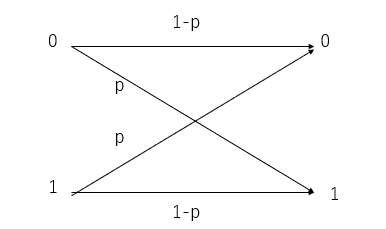
\includegraphics[width=0.7\textwidth]{img/Fig1.png}
        \caption[sample image (png)]{通信路線図}
        \label{Fig2_1}
    \end{figure}


ここで、$0$が入力されると確率 $1-p$で$0$が出力され、確率$p$で$1$が出力されることがわかる。
一方$1$が入力されると確率$p$で$0$が出力され、確率1-pで$1$が出力される。


